\chapter{Diagnostics, goodness of fit and postestimation}\label{ch:postest}

A fitted ERGM raises two questions. Did the estimation work, that is, did the Monte Carlo fit converge and is the Markov chain trustworthy? And does the model describe the network, that is, does it reproduce features of the data that were not built into it? This chapter describes the tools for both, and the other postestimation commands. All output was produced with the Lazega model of Section~\ref{sec:lazega}.

\section{Diagnosing the Markov chain: \texttt{estat mcmcdiag}}\label{sec:mcmcdiag}

\begin{lstlisting}
estat mcmcdiag [, plot name(string) pvalue(#) eps(#)]
\end{lstlisting}
\texttt{estat mcmcdiag} reports diagnostics of the \emph{final} Markov chain sample that the Monte Carlo fit simulated at its last coefficients. It is available after Monte Carlo maximum likelihood (and contrastive divergence and stochastic approximation), not after a pure pseudolikelihood fit, which involves no sampling; and it needs \texttt{e(mcmcsample)}, so it is not available after \opt{nomcmcsample}. It prints three blocks.

\paragraph{1.\ A summary per statistic.} The mean, standard deviation, lag-1 autocorrelation and effective sample size (ESS) of each model statistic in the sample, the acceptance rate of the sampler, and the burn-in and interval. The interval shown is that of the final sample, \texttt{e(mcmc\_interval\_final)}: in an adaptive fit the sampler may have lengthened it beyond the requested \texttt{e(mcmc\_interval)}, which is then named on a second line (``Requested interval''); the lags of the autocorrelation table below are multiples of the interval shown (Section~\ref{sec:lazega}). Before version 1.3.1 the header showed the requested interval, and \texttt{quietly estat mcmcdiag} printed the rows flagged by Geweke's test. The ESS is computed as \texttt{coda}'s \texttt{effectiveSize()} does, $n\,\mathrm{var}(x)$ divided by the spectral density at frequency zero estimated from an autoregressive model; the formula $n(1-\rho_1)/(1+\rho_1)$ would overstate the ESS severalfold for the slowly decaying autocorrelation typical of ERGM chains. The fit samples until the effective sample size of the estimating equations reaches a target (64 by default, \opt{mcmleeffectivesize()}), so that a final sample of a few hundred draws with an ESS of 64 to 100 is normal and is what \ergm{} produces; an ESS far below that, or a small fraction of the number of draws, means that the chain mixes slowly and that the estimates and standard errors carry a large Monte Carlo error.

\paragraph{2.\ Two convergence tests.} \emph{Geweke's diagnostic} compares the mean of the first 10\% of the retained sample with the mean of the last 50\%, each corrected for autocorrelation by the same autoregressive spectral estimate that enters the standard errors; $|z|>1.96$ (flagged with an asterisk) rejects stationarity of that statistic at the 5\% level. The \emph{Heidelberger--Welch test} first checks stationarity (a Cram\'er--von Mises test on the cumulative-sum path of the chain, discarding an increasing initial part of up to 50\%; \emph{Start} is the first retained draw once the test is passed and \emph{FAILED} means no part achieved it), and only then, for the retained part, whether the half-width of the 95\% confidence interval of the mean is within \opt{eps()} (default 10\%) of the mean. \opt{pvalue()} sets the level and must be 0.10, 0.05 (default), 0.025 or 0.01, because the test is evaluated against a table of critical values. Both tests are those of the \texttt{coda} package, which \ergm{} uses.

\paragraph{3.\ The report of R's diagnostics.} The rest of the output follows the report of R's \texttt{mcmc.diagnostics()}: the mean, standard deviation, naive and time-series standard error of the sample statistics centered at the observed statistics; their quantiles; a test of whether the sample statistics differ from the observed ones, with Hotelling's omnibus test; the cross-correlations; the autocorrelations at lags that are multiples of the interval; and the Geweke statistic with individual and joint $p$-values. (The multivariate spectral estimate follows \ergm{}~\ergmver{}; the development version of \ergm{} changes the estimator, so the omnibus $p$-values can differ in the second or third digit from those of a later release.) The matrices are returned in \texttt{r(mc\_summary)}, \texttt{r(mc\_quantiles)}, \texttt{r(mc\_obstest)}, \texttt{r(mc\_crosscorr)}, \texttt{r(mc\_autocorr)} and \texttt{r(mc\_geweke)}, and the first block in \texttt{r(ess)}, \texttt{r(geweke)}, \texttt{r(heidel)} and \texttt{r(acceptrate)}.

\paragraph{What to conclude.} \texttt{estat mcmcdiag} never claims that a fit converged merely because estimation stopped. The convergence test of the fit is a necessary check, not a proof: a low ESS, a low acceptance rate, a strongly autocorrelated chain, a large Geweke $z$ or a failed stationarity test are all reasons to refit with a higher target effective sample size (\opt{mcmleeffectivesize()}, the advice of the end note for an adaptive fit) or, for a fit with fixed-size samples (\opt{mcmleeffectivesize(0)}), a larger \opt{mcmcsamplesize()} or a longer \opt{mcmcinterval()}, even when \texttt{e(converged)} is 1. Section~\ref{sec:lazega} shows the output for the default settings and for a fit with a larger target. \opt{plot} draws a trace plot and a kernel density for each statistic in one figure (Figure~\ref{fig:mcmcdiag}); a trace that drifts or shows long runs at one level, rather than a stationary ``fuzzy caterpillar'', indicates poor mixing even when the numbers look acceptable. The diagnostics are those of the last round of simulation, before the final estimates were computed, and may understate the performance of the final model; to assess the final model on its own statistics, use \texttt{estat gof}.

\begin{figure}[ht]\centering
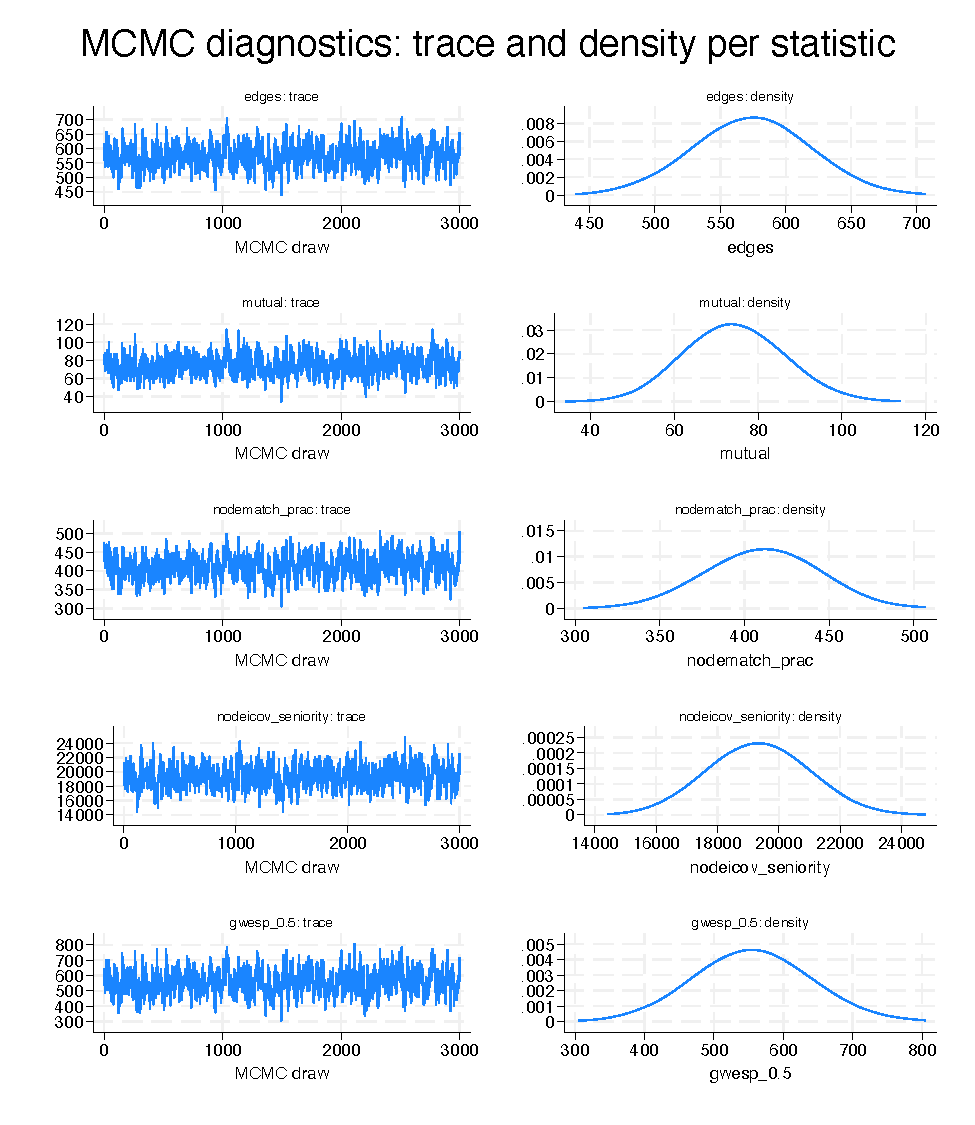
\includegraphics[width=0.8\textwidth]{fig/mcmcdiag.pdf}
\caption{\texttt{estat mcmcdiag, plot} for the Lazega model with the default settings: trace (left) and density (right) of the five model statistics in the final Monte Carlo sample.}\label{fig:mcmcdiag}
\end{figure}

\section{Goodness of fit: \texttt{estat gof}}\label{sec:gof}

\begin{lstlisting}
estat gof [, gof(statistics) nsim(#) seed(#) gofburnin(#) gofinterval(#) plot maxdeg(#) maxdist(#) name(string)]
\end{lstlisting}
A model is not validated by a significant coefficient; it is validated by whether networks simulated from it resemble the observed network on features that the model does not contain (Hunter, Goodreau and Handcock~\cite{hunter2008jasa}). \texttt{estat gof} follows R's \texttt{gof()}. It simulates the fitted model \opt{nsim()} times (default 100) --- continuing the Markov chain from the last network of the fit, with the burn-in and interval of the fit (the interval rescaled by sample size over \opt{nsim()} as in R; 3000 and 50 after a pseudolikelihood fit) --- and for each statistic reports the observed value, the minimum, mean and maximum over the simulations, and the Monte Carlo $p$-value $2\min\{P(\text{sim}\ge\text{obs}),P(\text{sim}\le\text{obs})\}$. Rows that are zero in every simulation and in the data are left out. \opt{gof(statistics)} chooses among
\begin{center}\footnotesize
\begin{tabular}{@{}ll@{}}\toprule
statistic & what is compared\\\midrule
\texttt{model} & the statistics of the model itself\\
\texttt{degree} & degree distribution (undirected networks)\\
\texttt{idegree}, \texttt{odegree} & in- and out-degree distributions (directed networks)\\
\texttt{b1degree}, \texttt{b2degree} & degree distributions of the two modes (two-mode networks)\\
\texttt{espartners} & edgewise shared partners\\
\texttt{dspartners} & dyadwise shared partners\\
\texttt{distance} & minimum geodesic distances (\texttt{Inf} for unreachable pairs)\\
\texttt{triadcensus} & triad census\\\bottomrule
\end{tabular}
\end{center}
A minus sign drops the model block (\opt{gof(idegree -model)}). The default is R's default for the type of network: for an undirected network \texttt{degree espartners distance model}, for a directed network \texttt{idegree odegree espartners distance model}, and for a two-mode network \texttt{b1degree b2degree dspartners distance model}. The tables are returned as matrices \texttt{r(gof\_}\emph{statistic}\texttt{)}, with the columns observed, minimum, mean, maximum and $p$-value; the older summary values (\texttt{r(obs\_meandeg)}, \texttt{r(sim\_avgpath)}, \texttt{r(obs\_triad\_}\emph{cat}\texttt{)}, \ldots) are still returned. The observed columns of these tables equal those of R's \texttt{gof()} for the Florentine (undirected) and Sampson (directed) networks.

\paragraph{How to read it.} A large systematic gap between the observed value and the range of the simulations is evidence against the model on that feature; a small $p$-value on one row among many rows is expected by chance, and the Monte Carlo $p$-values of neighboring rows are not independent. A network in which the observed count is 0 and the simulations are rarely 0 (or the reverse) at the end of a distribution is a typical sign of a missing term. The comparison is as noisy as the Markov chain: each simulated network is \opt{gofinterval()} proposals after the previous one, so that for a slowly mixing model even 100 draws can be too few, and refitting at different seeds can move the simulated mean degree from below the observed value to above it purely from Monte Carlo noise. If the final sample of the fit has a high autocorrelation, increase \opt{nsim()} (and consider \opt{gofinterval()}) before treating one run as a stable estimate; R's \texttt{gof()} has the same limitation. \opt{plot} draws the degree and geodesic-distance distributions: a whisker (minimum--maximum), a box (interquartile range) and a median marker summarize the simulated draws at each value, and the observed proportion is overlaid as a dashed line with triangle markers (Figure~\ref{fig:gof}). Degrees above \opt{maxdeg()} are pooled in one category and unreached pairs in a category \emph{NR}, as in statnet.

\begin{figure}[ht]\centering
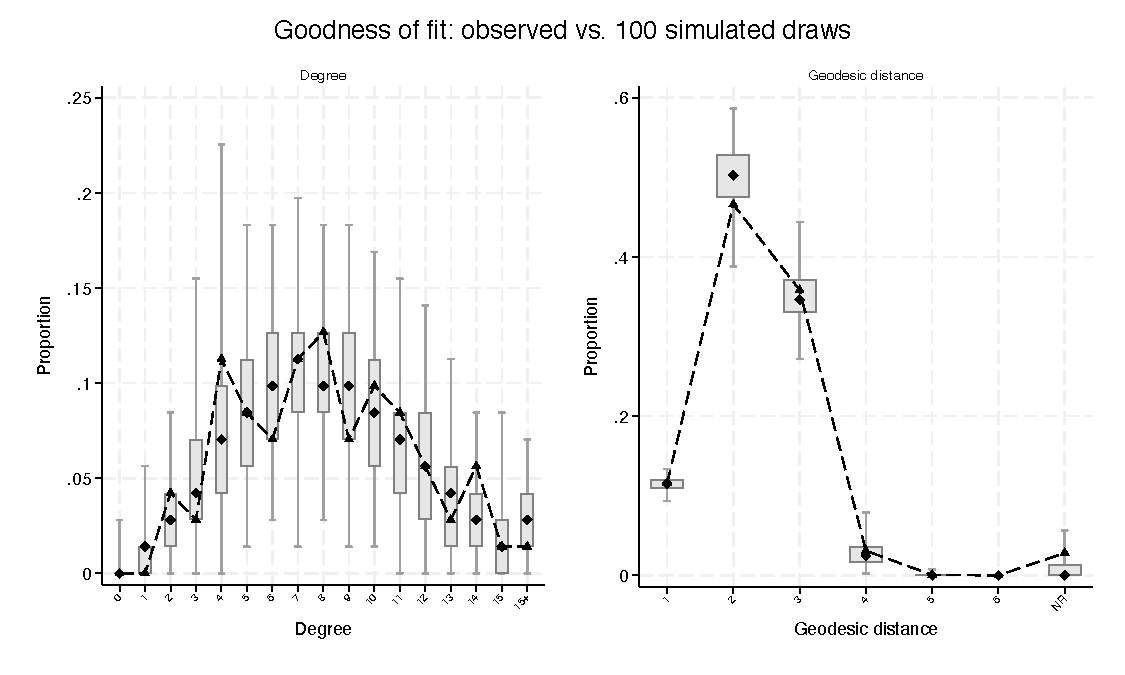
\includegraphics[width=0.85\textwidth]{fig/gof.pdf}
\caption{\texttt{estat gof, plot} for the Lazega model: degree and geodesic-distance distributions of 100 simulated networks (boxes) and of the observed network (line).}\label{fig:gof}
\end{figure}

\section{Information criteria and likelihood-ratio tests}\label{sec:ic}

After every fit \nwergm{} stores the log-likelihood as R's \texttt{logLik()} (Section~\ref{sec:loglik}). \texttt{estat ic} displays the number of informative dyads, the log-likelihood of the null model and of the fitted model, the degrees of freedom, AIC and BIC; it refuses when \texttt{e(ll)} is missing (a curved Monte Carlo fit, or \opt{nologlik}). \texttt{estimates stats} lists the criteria of several stored models; note that Stata's \texttt{estimates stats} uses the number of observations $N$ for the BIC, which for an ERGM is the number of informative dyads, as \texttt{estat ic} does. \texttt{lrtest} works between nested fits of the same network with the same number of informative dyads, for example
\begin{lstlisting}
. estimates store m1
. nwergm lazega_fr, edges mutual nodematch(prac) gwesp(0.5) ...
. estimates store m2
. lrtest m2 m1
\end{lstlisting}
The test is exact only to the extent that the log-likelihoods are: for Monte Carlo fits they carry the Monte Carlo standard error \texttt{e(ll\_se)}, which should be small compared with the differences that matter; for a pseudolikelihood fit of a dyad-dependent model the ``log-likelihood'' is the pseudolikelihood and a likelihood-ratio test is not valid. Wald tests of coefficients (\texttt{test}, \texttt{lincom}) work on \texttt{e(b)} and \texttt{e(V)}. Section~\ref{sec:comparing} has an example.

\section{Prediction: \texttt{predict}}\label{sec:predict}

\texttt{predict, matrix(}\emph{name}\texttt{)} [\opt{pr}|\opt{xb}] and \texttt{predict, frame(}\emph{name}\texttt{)} [\opt{pr}|\opt{xb}] give the conditional probability (\opt{pr}, the default) or the conditional log odds (\opt{xb}) of each informative dyad given the rest of the observed network, as R's \texttt{predict.ergm()} (equation~\eqref{eq:condlogit}). The frame has one row per dyad (\texttt{tail}, \texttt{head}, \texttt{p}); the matrix is $n\times n$ with missing dyads set to missing. The prediction is available for the most recent \texttt{nwergm} fit only. R uses the last network of the Monte Carlo sample as the basis for a dyad-dependent fit; \nwergm{} always uses the observed network. For a dyad-independent fit the two coincide, and the result equals R's to $10^{-7}$.

\section{Stored results}\label{sec:stored}

After a fit \texttt{nwergm} stores the following in \texttt{e()}. The listings in Section~\ref{sec:flo_ereturn} show them for a pseudolikelihood fit and for a Monte Carlo fit.

\paragraph{Scalars.}
\footnotesize
\begin{longtable}{@{}>{\raggedright\arraybackslash}p{4.7cm}>{\raggedright\arraybackslash}p{11.0cm}@{}}
\toprule
\texttt{e(N)} & Number of informative dyads (observed, not missing, not constrained).\\
\texttt{e(nodes)}, \texttt{e(ties)} & Number of nodes and of observed ties.\\
\texttt{e(nmissing)} & Number of missing dyads.\\
\texttt{e(ll)}, \texttt{e(ll\_0)} & Log-likelihood and null log-likelihood (Section~\ref{sec:loglik}). Missing after a curved Monte Carlo fit and with \opt{nologlik}.\\
\texttt{e(ll\_se)} & Monte Carlo standard error of \texttt{e(ll)} (0 when exact).\\
\texttt{e(df\_m)}, \texttt{e(rank)}, \texttt{e(df\_resid)} & Estimated coefficients (offsets excluded), rank, and $N-$\texttt{df\_m}.\\
\texttt{e(deviance)}, \texttt{e(deviance\_0)} & Residual and null deviance, $-2$ times the log-likelihood.\\
\texttt{e(aic)}, \texttt{e(bic)} & AIC and BIC (BIC with $N$ the number of informative dyads).\\
\texttt{e(curved)} & 1 if the model has a curved term.\\
\texttt{e(native)} & 1 if the native plugin was used (the sampler for Monte Carlo fits, the design-matrix build for pseudolikelihood fits), 0 for Mata. Informational only.\\
\texttt{e(spcache)} & 1 if \opt{spcache} was used.\\
\texttt{e(converged)} & 1 if the convergence test of the Monte Carlo iteration was satisfied (Monte Carlo fits only).\\
\texttt{e(mcmle\_iterations)} & Number of outer iterations (for stochastic approximation: of phase 2).\\
\texttt{e(mcmc\_acceptrate)} & Acceptance rate of the final simulation.\\
\texttt{e(mcmc\_burnin)}, \texttt{e(mcmc\_interval)}, \texttt{e(mcmc\_samplesize)} & Burn-in and interval as requested, and the number of draws kept by the last iteration (in the adaptive sample, more than the base size \opt{mcmcsamplesize()} if the effective sample size target needed it).\\
\texttt{e(mcmc\_interval\_final)} & The interval of the sample of the last iteration. In the adaptive sample (the default) it follows from the halving of the interval between iterations and the thinning of the sample (Section~\ref{sec:adaptive}) and can be shorter or longer than \texttt{e(mcmc\_interval)}; in a fixed-size fit it is larger than \texttt{e(mcmc\_interval)} if the interval was grown.\\
\bottomrule
\end{longtable}
\normalsize

\paragraph{Macros.}
\footnotesize
\begin{longtable}{@{}>{\raggedright\arraybackslash}p{4.7cm}>{\raggedright\arraybackslash}p{11.0cm}@{}}
\toprule
\texttt{e(cmd)} & \texttt{nwergm}\\
\texttt{e(title)} & Title of the estimation.\\
\texttt{e(depvar)} & Name of the fitted network.\\
\texttt{e(method)} & \texttt{mple} or \texttt{mcmle} (the simulation-based estimators share \texttt{mcmle}).\\
\texttt{e(estimate)} & \texttt{MLE}, \texttt{CD} or \texttt{SA} for a simulation-based fit (empty after a pseudolikelihood fit).\\
\texttt{e(directed)} & \texttt{true} or \texttt{false}.\\
\texttt{e(proposal)} & Proposal used (simulation-based fits).\\
\texttt{e(ll\_method)} & How \texttt{e(ll)} was obtained: \texttt{exact}, \texttt{pseudolikelihood} or \texttt{bridge sampling}.\\
\texttt{e(version)} & The release of \nwergm{} that produced the results.\\
\texttt{e(predict)}, \texttt{e(estat\_cmd)}, \texttt{e(properties)} & Postestimation dispatch.\\
\bottomrule
\end{longtable}
\normalsize

\paragraph{Matrices.} \texttt{e(b)} (coefficients) and \texttt{e(V)} (covariance matrix); \texttt{e(mcmcsample)}, the final simulation's sample of the model statistics, size $\times$ number of coefficients (simulation-based fits, unless \opt{nomcmcsample}); \texttt{e(obs\_stats)}, the observed statistics (pseudolikelihood fits).

\paragraph{\texttt{r()}.} \texttt{estat mcmcdiag}, \texttt{estat gof}, \texttt{nwergm simulate} and \texttt{nwergm version} return the results named in the sections above: \texttt{r(ess)}, \texttt{r(geweke)}, \texttt{r(heidel)}, \texttt{r(acceptrate)} and \texttt{r(mc\_}\ldots\texttt{)}; \texttt{r(gof\_}\emph{statistic}\texttt{)}, \texttt{r(nsim)}, \texttt{r(burnin)}, \texttt{r(interval)}; \texttt{r(stats)} (\texttt{nwergm simulate}, also \texttt{r(nsim)}, \texttt{r(burnin)}, \texttt{r(interval)}); \texttt{r(version)}, \texttt{r(date)}, \texttt{r(core)}, \texttt{r(plugin)}, \texttt{r(reference)}, \texttt{r(license)}.
